\chapter{Vývojová dokumentácia}
\label{vyvojova dokumentacia}

V~tejto kapitole sa pozrieme na~implementáciu nášho~systému. Zameráme sa na~organizáciu a~implementáciu dôležitých častí aplikácie. Cieľom tohto textu nie je opísať správanie každého riadka kódu. Na~to slúži kód samotný~(prípadne komentáre, ktoré autor pridal na~miesta, kde to uznal za~vhodné). Kód aplikácie sa nachádza v~elektronickej prílohe (pre~prehľad obsahu elektronickej prílohy viď~\ref{prehlad elektronickych priloh}) alebo~je taktiež možné vidieť kód aplikácie v~online repozitári (viď~odkaz v~prílohe~\ref{implementacia}). Náš systém sa skladá z~dvoch projektov~-- ServISWebApp a~ServISData (viď~obr.~\ref{architektura systemu}).

\begin{figure}[H]\centering
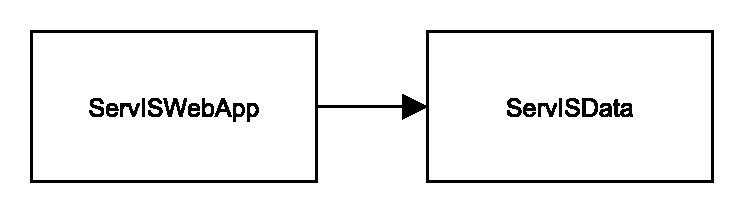
\includegraphics[width=140mm]{../img/architektura systemu}
\caption{Architektúra systému.}
\label{architektura systemu}
\end{figure}

Zmyslom projektu ServISData je správa databázových entít a~komunikácia s~databázou. Projekt ServISWebApp predstavuje rozhranie pre~užívateľov, a~zároveň obsahuje logiku nášho~systému. ServISWebApp využíva ServISData, aby sa dostal k dátam, ktoré potom môže užívateľom napr. zobrazovať. Navyše projekt ServISWebApp je rozdelený na dve časti~-- frontendová a backendová časť (rozdelenie bolo spomenuté v podkap. \ref{rozdelenie na frontendovu a backendovu cast}).

\newpage

\section{Adresárová štruktúra systému}

V tejto podkapitole sa pozrieme na adresárovú štruktúru systému a~povieme si na~čo slúžia jednotlivé priečinky, resp.~súbory v~nich. Priečinky označené \textcolor{blue}{modrou} farbou patria do~frontendovej časti a~priečinky označené \textcolor{red}{červenou} farbou patria do~backendovej časti projektu ServISWebApp.
\\

\dirtree{%
.1 ServISWebApp.
.2 Súbory v koreňovom priečinku projektu ServISWebapp~-- kód slúžiaci (zväčša) na~konfiguráciu a~spustenie programu.
.2 \textcolor{red}{Auth}~-- triedy slúžiace na~autentifikáciu užívateľa.
.2 \textcolor{red}{BackgroundServices}~-- triedy procesov bežiacich na pozadí.
.2 \textcolor{blue}{Components}~-- komponenty využívané na stránkach z~prieč.~\texttt{Pages}.
.3 \textcolor{blue}{Buttons}~-- komponenty reprezentujúce rôzne tlačidlá.
.3 \textcolor{blue}{Forms}~-- komponenty reprezentujúce formuláre.
.3 \textcolor{blue}{Managements}~-- obsahuje komponentu pre správu bagrov, prídavných zariadení atď..
.2 \textcolor{blue}{CssProviders}~-- triedy zodpovedné za zmenu kaskádových štýlov vo formulároch.
.2 \textcolor{blue}{Pages}~-- stránky zložené z~komponentov z~priečinku~\texttt{Components}.
.3 \textcolor{blue}{Admin}~-- stránky určené výhradne pre~administrátorov.
.2 \textcolor{red}{Shared}~-- pomocné triedy využívané z rôznych miest programu.
.3 \textcolor{red}{Extensions}~-- obsahuje triedu s extension metódami.
}

\dirtree{%
.1 ServISData.
.2 Súbory v koreňovom priečinku projektu ServISData~-- obsahuje kód pre prácu s~databázou, rozhranie projektu ServISData, a~takisto ďalší pomocný kód pre prácu s~modelmi (triedy nachádzajúce sa v~priečinku \texttt{Models}).
.2 Attributes~-- atribúty modelov (triedy, ktoré sa nachádzajú v~priečinku~\texttt{Models}).
.2 DataOperations~-- kód určený pre~vykonávanie operácií s~dátami (napr.~filtrovanie, stránkovanie atď.).
.2 Interfaces~-- rozhrania (napr.~rozhranie~\texttt{IItem}, ktoré spĺňajú všetky modely (triedy nachádzajúce sa v~priečinku \texttt{Models}).
.2 Migrations~-- priečinok vygenerovaný frameworkom EF Core obsahujúci migrácie~\cite{migrations}.
.2 Models~-- obsahuje modely (triedy reprezentujúce databázové entity).
}

\section{Backendová časť}

Backendová časť pokrýva logiku aplikácie mimo logiky užívateľského rozhrania, napr. vyhodnocovanie dražieb v~aukcii. V tejto kapitole si prejdeme niektoré (významnejšie) z~tried backendovej časti, ktoré sú využívané frontendovou časťou aplikácie.

\subsection{Trieda CustomAuthenticationStateProvider}
\label{trieda customauthenticationstateprovider}

Táto trieda poskytuje metódy pre registráciu a~prihlásenie užívateľa do~systému. Takisto poskytuje metódy pre~získanie informácií o~prihlásenom užívateľovi.

\subsection{Trieda PasswordHasher}
\label{trieda passwordhasher}

Trieda obsahuje metódy na prácu s hashami. Umožňuje hashovať heslá, a~tiež určovať, či hash patrí heslu.

\subsection{Trieda ServISApi a~rozhranie IServISApi}
\label{trieda servisapi a rozhranie iservisapi}

Trieda \verb|ServISApi| predstavuje rozhranie (API~\cite{api}) projektu~ServISData. Poskytuje metódy pre vytváranie/úpravu, mazanie a~získavanie dát entít databázy opísaných v~časti Návrh relačného modelu databázy (viď~\ref{navrh relacneho modelu databazy}). Táto trieda je implementáciou rozhrania~\verb|IServISApi|. Pri~registrácií \verb|IServISApi| medzi služby, v~súbore~Program.cs, je ako implementácia tohto rozhrania dosadená trieda~\verb|ServISApi|. Preto keď z nejakého komponentu žiadame \verb|IServISApi|, framework (dependency injection) nám poskytne inštanciu triedy~\verb|ServISApi|.

\subsection{Trieda DataOperations}
\label{trieda dataoperations}

Trieda \verb|DataOperations| sa využíva pre~filtrovanie, zoradzovanie, stránkovanie alebo~vyhľadávanie dát. V~tejto triede existuje vnorená trieda~\verb|Configuration|, ktorá slúži pre~nastavenie spomínaných operácií (napr.~s jej pomocou vieme nastaviť, aby zoradenie dát bolo zostupne). Pomocou triedy~\verb|Configuration| je možné vytvoriť inštanciu triedy~\verb|DataOperations|, a~tú je potom možné využiť v~metódach, ktoré vracajú dáta (resp.~kolekciu dát), napr.~\verb|DataOperations| sa využíva ako voliteľný parameter v~niektoých metódach pre~získavanie dát spomenutých v~predchádzajúcej časti textu (viď~\ref{trieda servisapi a rozhranie iservisapi}).

\subsection{Trieda EmailManager}
\label{trieda emailmanager}

Táto trieda poskytuje rôzne metódy pre~prácu s~emailami. Pomocou nej je možné napr.~posielať emaily, získavať emaily z~Gmailovej schránky, mazať emaily atď.

\subsection{Trieda TimerService a~jej potomkovia}
\label{trieda timerservice}

Trieda \verb|TimerService| je abstraktnou triedou, ktorá zakrýva prácu s~triedou \verb|Timer|. Umožňuje svojím potomkom definovať čo sa má vykonávať a~v~akom intervale.

Trieda \verb|EverySecondTimerService| je potomkom triedy~\verb|TimerService|. Umožňuje svojím užívateľom (iným triedam) registrovať akciu, ktorá sa má vykonávať každú sekundu. V~aplikácii sa využíva pre~zobrazovanie odpočtu do~konca aukčných ponúk (dražieb).

Trieda \verb|AuctionEvaluatorService| je ďalším potomkom triedy~\verb|TimerService|. Každú minútu skontroluje všetky aukčné ponuky a~tie, ktoré už skončili vyhodnotí (vyhodnocovanie už bolo opísané v~podkapitole~\ref{aukcia odpocet a vyhodnocovanie}).

\section{Frontendová časť}

Frontendová časť má na~starosti prezentovanie dát a~interakciu s~užívateľom. V~tejto kapitole si prejdeme jednotlivé stránky webu a~opíšeme si aké významnejšie triedy (komponenty) sa v~nich využívajú.

\subsection{Zobrazovanie obsahu podľa roly}
\label{zobrazovanie obsahu podla roly}

Z požiadavky P1 (Roly užívateľa, viď v podkap.~\ref{poziadavky}) vieme, že systém má rozlišovať medzi bežným zákazníkom a administrátorom, a~podľa toho mu upraviť obsah na stránke. Z kapitoly Návrh užívateľského rozhrania (viď~\ref{navrh ui}) vieme, že by mali existovať stránky, kde sa zobrazujú/schovávajú len určité časti. Napríklad v navigácii (viď~vľavo na~obr.~\ref{layout}) by sa mal zobraziť odkaz \uv{Správa webu} iba administrátorom. Ale takisto existujú aj prípady, kedy by sme chceli obmedziť prístup na celú stránku. Napr. chceme, aby sa mohol na~stránku pre~vytvorenie (alebo úpravu) hlavnej ponuky (viď obr. \ref{main offer form}) mohol dostať iba administrátor.

Platforma .NET nám na to ponúka triedu~\texttt{AuthorizeView}~\cite{authorizeview}, presnejšie ide o komponent, pomocou ktorého vieme špecifikovať aký obsah (a komu, akej role) sa má zobraziť na~stránke. Takže napríklad v prípade navigácie vyzerá implementácia takto:

\begin{verbatim}
...
<div class="nav-item px-3">
    <NavLink ... href="kontakt">
        <span class="oi oi-plus" ..."></span> Kontakt
    </NavLink>
</div>
<AuthorizeView Roles="Administrator">
    <div class="nav-item px-3">
        <NavLink ... href="admin">
            <span class="oi oi-cog" ...></span> Správa webu
        </NavLink>
    </div>
</AuthorizeView>
...
\end{verbatim}

V prípade obmedzenia celej stránky využívame atribút~\texttt{[Authorize]}~\cite{authorize attribute}. Takže stačí ak do~implementácie, napr.~spomínanej stránky pre~vytvorenie (alebo~úpravu) hlavnej ponuky, dopíšeme atribút \verb|[Authorize]| následovne:

\begin{verbatim}
@page "/admin/nova-ponuka"
@page "/admin/uprava-ponuky/{MainOfferId:int}"

@attribute [Authorize(Roles = "Administrator")]
...
\end{verbatim}

\subsection{Hlavné rozloženie stránky}
\label{hlavne rozlozenie stranky}

Za hlavné rozloženie stránky, ktoré bolo navrhnuté v~časti~Hlavné rozloženie aplikácie (viď~\ref{hlavne rozlozenie aplikacie}), je zodpovedný komponent~\verb|MainLayout|. V~rámci tohto komponentu sme využili komponent~\texttt{SfDialogProvider}~\cite{sfdialogprovider}, ktorý nám umožní využívať potvrdzovacie modálne okná (tie si opíšeme v~následujúcej časti textu, viď \ref{modalne potvrdzovacie okno2}). Okrem toho sa v~komponente~\verb|MainLayout| využíva komponent~\verb|NavMenu| (navigácia), a~ten v sebe obsahuje komponenty \verb|NavLink| (predstavujú odkazy v navigácii), \verb|AuthorizeView| (viď~\ref{zobrazovanie obsahu podla roly}) a~\verb|LoginPanel|.

Komponent~\verb|LoginPanel| slúži v prípade neprihláseného užívateľa na~presmerovanie na stránky s formulármi pre prihlásenie alebo registráciu. V prípade prihláseného užívateľa slúži na~presmerovanie na~profil alebo~na~odhlásenie. Využíva preto komponent~\verb|AuthorizeView| (viď~\ref{zobrazovanie obsahu podla roly}) a~triedu \verb|CustomAuthenticationStateProvider| (viď~\ref{trieda customauthenticationstateprovider}).

\subsection{Modálne potvrdzovacie okno}
\label{modalne potvrdzovacie okno2}

V predchádzajúcej časti textu (viď \ref{hlavne rozlozenie stranky}) bolo v~súvislostii s~komponentom \verb|SfDialogProvider| spomenuté potvrdzovacie modálne okno. Potvrdzovacie modálne okno bolo navrhnuté v~podkapitole Modálne potvrdzovacie okno (viď \ref{modalne potvrdzovacie okno}) a~naimplementované v triede \verb|Modals| za~pomoci služby (triedy)~\texttt{SfDialogService}~\cite{sfdialogservice}.

\subsection{Stránky s~podmienkami používania a~zásadami ochrany osobných údajov}

V podkapitole Sekcie Podmienky používania a~Zásady ochrany osobných údajov (viď \ref{gdpr}) boli navrhnuté stránky s~podmienkami používania a~zásadami ochrany osobných údajov. Implementáciu týchto stránok môžeme nájsť v~súboroch \verb|Terms.razor| a~\verb|PrivacyPolicy.razor|.

\subsection{Stránka s hlavnou ponukou (domovská stránka)}

Implementáciu časti aplikácie s vylistovanými kartami hlavnej ponuky (slúži ako domovská stránka), ktorá bola navrhnutá v časti Hlavná ponuka (viď~\ref{hlavna ponuka}), môžeme nájsť v~súbore~\verb|Index.razor|. Stránka využíva komponenty \verb|AuthorizeView| (viď \ref{zobrazovanie obsahu podla roly}) a~\verb|MainCard| (tento komponent predstavuje kartu hlavnej ponuky). Kód tejto stránky využíva pre získanie dát o hlavných ponukách (reprezentované triedou \verb|MainOffer|) rozhranie (API) projektu ServISData (viď \ref{trieda servisapi a rozhranie iservisapi}).

\subsection{Stránka pre vytvorenie a úpravu hlavnej ponuky}

Obe stránky, stránka pre vytvorenie novej, ale aj stránka pre úpravu existujúcej hlavnej ponuky (navrhnuté v~časti~\ref{vytvorenie novej a uprava existujucej hlavnej ponuky}), sú naimplementované v~súbore~\verb|CreateMainOffer.razor|. Implementácia tejto stránky využíva atribút~\verb|[Authorize]| (viď~\ref{zobrazovanie obsahu podla roly}) a~komponent~\verb|MainOfferForm| (formulár pre~vytváranie/úpravu hlavnej ponuky, ktorá je v~kóde reprezentovaná triedou \verb|MainOffer|). Komponent \verb|MainOfferForm|) využíva pre výber typu bagra (v~kóde reprezentovaný triedou \verb|ExcavatorType|) komponent \verb|ItemsSelector|. V prípade, že ide o~úpravu existujúcej hlavnej ponuky, jej dáta sa načítajú pomocou rozhrania projektu ServISData (viď \ref{trieda servisapi a rozhranie iservisapi}) a~predajú formuláru.

\subsection{Stránka s ponukou (nových) bagrov}

Návrh tejto časti aplikácie bol opísaný v časti textu Ponuka (nových) bagrov (viď~\ref{ponuka novych bagrov}). Implementácia stránky sa nachádza v~súbore~\verb|Excavators.razor| a~obsahuje komponenty~\verb|AuthorizeView| (viď~\ref{zobrazovanie obsahu podla roly}) a~\verb|ExcavatorLister|. Pomocou rozhrania projektu ServISData (viď \ref{trieda servisapi a rozhranie iservisapi}) sa získajú objekty typu \verb|Excavator| reprezentujúce bagre a~predajú sa už spomínanej komponente \verb|ExcavatorLister| na~vylistovanie~-- pre každý bager sa zobrazí karta bagra (komponent \verb|ExcavatorCard|). V návrhu tejto časti aplikácie bolo tiež spomenuté, že sa majú vylistovať karty bagrov určitého typu, ktoré neboli určené iba pre~aukciu. Dosiahli sme toho pomocou tried \verb|DataOperations| a (jej vnorenej triedy) \verb|Configuration|, ktoré implementácia stránky taktiež obsahuje (tieto triedy boli spomenuté už skôr v časti~\ref{trieda dataoperations}).

\subsection{Stránka s ponukou prídavných zariadení}

Návrh tejto stránky sa nachádza v časti textu Ponuka prídavných zariadení (viď \ref{ponuka pridavnych zariadeni}). Implementácia stránky sa nachádza v~súbore \linebreak\verb|AdditionalEquipments.razor| a~obsahuje komponenty~\verb|AuthorizeView| (viď~\ref{zobrazovanie obsahu podla roly}) a~\verb|AdditionalEquipmentLister|. Komponent \linebreak\verb|AdditionalEquipmentLister| slúži na~vylistovanie kariet prídavných zariadení (komponenty \verb|AdditionalEquipmentCard|), dáta prídavných zariadeniach (reprezentované triedami \verb|AdditionalEquipment|) získava z~rozhrania projektu ServISData (viď \ref{trieda servisapi a rozhranie iservisapi})

\subsection{Stránka s~detailom bagra, prídavného zariadenia}

Táto časť aplikácie bola navrhnutá v časti Detail bagra, prídavného zariadenia (viď \ref{detail bagra pridavneho zariadenia}). Implementáciu stránky s detailom bagra môžeme nájsť v~súbore~\verb|ExcavatorDetail.razor| a~implementáciu stránky s detailom prídavného zariadenia môžeme nájsť v~súbore \verb|AdditionalEquipmentDetail.razor|. Obidve implementácie využívajú komponenty~\verb|AuthorizeView| (viď~\ref{zobrazovanie obsahu podla roly}), \verb|PhotoSlider| (pre zobrazenie fotiek) a~\verb|DemandForm| (formulár, ktorého návrh bol opísaný v časti \ref{dopyt}). Komponent~\verb|DemandForm| využíva na~odoslanie správy (emailu) triedu \verb|EmailManager| (viď~\ref{trieda emailmanager}). Ďalej obe implementácie stránok čerpajú dáta na~zobrazenie z~rozhrania projektu ServISData (viď \ref{trieda servisapi a rozhranie iservisapi}). V~prípade stránky s~detailom bagra sa získa trieda \verb|Excavator| (obsahujúca dáta bagra) a~v~prípade stránky s~detailom prídavného zariadenia sa získa trieda \verb|AdditionalEquipment| (obsahujúca dáta prídavného zariadenia).

\subsection{Stránka pre~vytvorenie a~úpravu bagra}
\label{stranka pre vytvorenie a upravu bagra}

Návrh tejto časti aplikácie môžeme nájsť v~časti textu~Vytvorenie nového a~úprava existujúceho bagra (viď~\ref{vytvorenie noveho a uprava existujuceho bagra}). Implementácia sa nachádza v~súbore \verb|CreateExcavator.razor| a~obsahuje atribút~\verb|[Authorize]| (viď~\ref{zobrazovanie obsahu podla roly}) a~komponent~\verb|ExcavatorForm|. V prípade, že ide o úpravu existujúceho bagra, sa pomocou rozhrania projektu ServISData (viď \ref{trieda servisapi a rozhranie iservisapi}) načítajú a~následne predajú dáta komponente~\verb|ExcavatorForm|. \verb|ExcavatorForm| je formulár pre~vytváranie/úpravu bagra (bager je reprezentovaný triedou~\verb|Excavator|). V návrhu je napísané, že do~formulára by malo byť možné nahrať viacero fotiek, vybrať typ bagra, a~tiež vybrať aké náhradné diely patria do~bagra. Kvôli tomu formulár obsahuje komponenty~\verb|InputItemPhotos| (pre~nahratie fotiek), \verb|ItemsSelector| (pre~výber typu bagra) a~\verb|ChecklistTable| (pre~výber náhradných dielov).

\subsection{Stránka pre~vytvorenie a~úpravu prídavného zariadenia}

Implementácia časti aplikácie, ktorá bola navrhnutá v~časti textu~Vytvorenie nového a~úprava existujúceho prídavného zariadenia (viď~\ref{vytvorenie noveho a uprava existujuceho pridavného zariadenia}), obsahuje atribút~\verb|[Authorize]| (viď~\ref{zobrazovanie obsahu podla roly}) a~komponent~\verb|AdditionalEquipmentForm|. V~prípade, že ide o~úpravu existujúceho prídavného zariadenia, sa pomocou rozhrania projektu ServISData (viď~\ref{trieda servisapi a rozhranie iservisapi}) načítajú a~následne predajú dáta komponente~\verb|AdditionalEquipmentForm|. \verb|AdditionalEquipmentForm| je formulár pre~vytváranie/úpravu prídavného zariadenia (prídavné zariadenie je reprezentované triedou~\verb|AdditionalEquipment|). V návrhu je napísané, že do~formulára by malo byť možné nahrať viacero fotiek, vybrať značku a kategóriu prídavného zariadenia, ale aj vybrať typ bagra, pre ktorý je prídavné zariadenie určené. Kvôli tomu formulár obsahuje komponenty~\verb|InputItemPhotos| (pre~nahratie fotiek) a~\verb|ItemsSelector| (túto komponentu obsahuje dokonca trikrát, pre~výber značky a~kategórie prídavného zariadenia, ale~tiež aj pre~výber typu bagra).

\subsection{Stránka s aukčnými ponukami}

Návrh stránky s aukčnými ponukami, ktorá bola navrhnutá v~časti~Aukčné ponuky (viď~\ref{aukcne ponuky}), sa nachádza v~súbore~\verb|AuctionOffers.razor|. Implementácia stránky využíva komponent~\verb|AuthorizeView| (viď~\ref{zobrazovanie obsahu podla roly}) a~na~vylistovanie kariet aukčných ponúk (komponentov typu \verb|AuctionOfferCard|, ktoré v~sebe obsahujú pre~zobrazenie odpočtu komponent~\verb|CountdownDisplayer| využívajúci triedu~\verb|EverySecondTimerService| spomenutú v~časti \ref{trieda timerservice}) využíva komponent~\verb|AuctionOffersLister|. \verb|AuctionOffersLister| získava dáta aukčných ponúk (reprezentované triedami typu \verb|AuctionOffer|) z~rozhrania projektu ServISData (viď~\ref{trieda servisapi a rozhranie iservisapi}).

\subsection{Stránka s detailom aukčnej ponuky}

Stránka s detailom aukčnej ponuky, ktorej návrh je opísaný v~časti~Detail aukčnej ponuky (viď \ref{detail aukcnej ponuky}), je implementovaná v~súbore~\verb|AuctionOfferDetail.razor|. Stránka využíva komponenty~\verb|AuthorizeView| (viď~\ref{zobrazovanie obsahu podla roly}), \verb|PhotoSlider| (pre zobrazenie fotiek), \verb|CountdownDisplayer| (pre~zobrazenie odpočtu, využíva na~to triedu~\verb|EverySecondTimerService| spomenutú v~časti \ref{trieda timerservice}) a~\verb|AuctionBidForm|. Stránka čerpá dáta aukčnej ponuky na~zobrazenie z~rozhrania projektu ServISData (viď \ref{trieda servisapi a rozhranie iservisapi}). Na~stránke sa tiež využíva trieda obsahujúca dáta o~aukčnej ponuke~-- \verb|AuctionOffer|. Okrem toho implementácia stránky obsahuje aj komponent \verb|AuctionBidForm|, ktorého návrh bol opísaný v~časti~\ref{ponukanie sumy do drazby}. Komponent~\verb|AuctionBidForm| je formulár, ktorý pracuje s triedou \verb|AuctionBid| (predstavuje zákazníkovú ponúknutú sumu do dražby).

\subsection{Stránka pre~vytvorenie a~úpravu aukčnej ponuky}

Obidve stránky, stránka pre vytvorenie novej, ale~aj stránka pre~úpravu existujúcej aukčnej ponuky (navrhnuté v~časti \ref{vytvorenie novej a uprava existujucej aukcnej ponuky}), sú naimplementované v~súbore \verb|CreateAuctionOffer.razor|. Implementácia tejto stránky využíva atribút~\verb|[Authorize]| (viď~\ref{zobrazovanie obsahu podla roly}) a~komponent~\verb|AuctionOfferForm| (formulár pre~vytváranie/úpravu aukčnej ponuky, ktorá je v~kóde reprezentovaná triedou \verb|AuctionOffer|). V~návrhu stránky je spomenuté, že formulár by mal umožniť výber bagra (v~kóde reprezentovaný triedou \verb|Excavator|) do~dražby~-- na~to \verb|AuctionOffer|) využíva komponent \verb|ItemsSelector|. V~prípade, že ide o~úpravu existujúcej aukčnej ponuky, jej dáta sa načítajú pomocou rozhrania projektu ServISData (viď \ref{trieda servisapi a rozhranie iservisapi}) a~predajú formuláru.

\subsection{Stránky Služby, Kontakt a~O~nás}

Návrh stránky Služby bol opísaný v~podkapitole~Splnenie P8 (viď~\ref{splnenie p8}). Implementáciu stránky môžeme nájsť v~súbore~\verb|Services.razor|, využíva komponent~\verb|DemandForm|.

Ďalej návrh stránok Kontakt a~O~nás bol opísaný v~podkapitole~Splnenie P9 (viď~\ref{splnenie p9}). Implementáciu stránky Kontakt môžeme nájsť v~súbore~\verb|Contact.razor| a~implementáciu stránky~O~nás môžeme nájsť v~súbore~\verb|About.razor|.

\subsection{Stránka pre správu webu}

V podkapitole Splnenie P5, P7 a~správa predmetov (viď \ref{splnenie p5 p7 a sprava predmetov}) bola navrhnutá emailová schránka a~časť aplikácie pre~správu obsahu webu (administrátorská stránka). Implementácia administrátorskej stránky sa nachádza v~súbore~\verb|AdministratorPage.razor| a~využíva atribút~\verb|[Authorize]| (viď~ref{zobrazovanie obsahu podľa roly}), komponent \verb|TabControl| s komponentmi \verb|TabPage| (tvoria panel s kartami Správy, Náhradné diely atď., viď~vrchnú časť obr.~\ref{messages}). 

Na karte Správy sa zobrazuje komponent \verb|Message|, ktorý v~sebe obsahuje komponenty \verb|ThreadsView| (pohľad s~vylistovanými konverzáciami, ktoré sú reprezentované komponentom \verb|ThreadRow|), \verb|ThreadView| (pohľad, ktorý sa zobrazí pri otvorení konverzácie, zobrazí správy v konverzácii reprezentované komponentmi typu \verb|Message|) a~\verb|MessageSettings| (pohľad, ktorý sa zobrazí pri prekliknutí do~časti s~nastaveniami správ, využíva rozhranie projektu ServISData, viď~\ref{trieda servisapi a rozhranie iservisapi} a~komponenty typu \verb|AutogeneratedMessageForm| pre~editáciu tvaru automaticky generovaných správ, ktoré sú v~kóde reprezentované triedou~\verb|AutogeneratedMessage|). Ďalej sa na~karte pre~získanie správ z~Gmailu využíva trieda \verb|EmailManager| (viď~\ref{trieda emailmanager}).

Ostatné karty (Náhradné diely, Bager atď.) zobrazujú komponent \verb|ItemsManagement|, ktorý predstavuje tabuľku opísanú v~časti \ref{karta nahradne diely}. \linebreak\verb|ItemsManagement| tiež využíva rôzne komponenty na~zobrazenie formulára podľa toho, na akej karte sa užívateľ nachádza. Teraz prejdeme zbytok kariet a~opíšeme si, aké komponenty využívajú:

\begin{itemize}
\item \textbf{Karta Náhradné diely}

Táto karta využíva komponent~\verb|SparePartForm|, ktorý predstavuje formulár pre vytváranie/úpravu prídavných zariadení~-- tie sú reprezentované triedami typu~\verb|SparePart|. V časti Karta Náhradné diely (viď~\ref{karta nahradne diely}) bolo spomenuté, že formulár by mal umožniť zadať do~akých bagrov náhradný diel patrí, a~preto \verb|SparePartForm| obsahuje komponent~\verb|ChecklistTable|, ktorý to umožňuje. Pre~získanie bagrov a~v~prípade upravovania existujúceho náhradného dielu pre získanie dát o~upravovanom náhradnom diele sa využíva rozhranie projektu ServISData (viď~\ref{trieda servisapi a rozhranie iservisapi}).

\item \textbf{Karta Bagre}

Ďalej táto karta využíva komponent~\verb|ExcavatorForm|, ktorý predstavuje formulár pre vytváranie/úpravu bagrov, ktoré sú reprezentované triedami typu~\verb|Excavator|. Komponet~\verb|ExcavatorForm| bol podrobnejšie opísaný v~časti Stránka pre~vytvorenie a~úpravu bagra (viď~\ref{stranka pre vytvorenie a upravu bagra}).

\item \textbf{Karta Typy bagrov}

Karta využíva komponent~\verb|ExcavatorTypeForm|, ktorý predstavuje formulár pre vytváranie/úpravu typov bagrov, a~tie sú reprezentované triedami typu~\verb|ExcavatorType|. V časti Karty Bagre, Typy bagrov, Typy vlastností bagrov (viď~\ref{karty bagre typy bagrov typy vlastnosti bagrov}) bolo spomenuté, že formulár by mal umožniť výber značky bagra a~kategórie bagra, a~preto \verb|ExcavatorTypeForm| obsahuje dva komponenty typu~\verb|ItemsSelector|, ktoré to umožňujú. Okrem toho bolo napísané, že by mal formulár umožniť výber typov vlastností, ktoré bude mať vytváraný (resp.~upravovaný) typ bagra. Kvôli tomu formulár tiež využíva komponent~\verb|ChecklistTable|. Pre~získanie typov vlastností a~v~prípade upravovania existujúceho typu bagra pre~získanie dát o~upravovanom type bagra sa využíva rozhranie projektu ServISData (viď~\ref{trieda servisapi a rozhranie iservisapi}).

\item \textbf{Karta Typy vlastností bagrov}

Tu sa využíva komponent~\verb|ExcavatorPropertyTypeForm| predstavujúci formulár pre vytváranie/úpravu typov vlastností bagrov, ktoré sú reprezentované triedami typu~\verb|ExcavatorPropertyType|.

\item \textbf{Karta Kategórie a~značky~bagrov}

Na tejto karte sa nachádzajú dve tabuľky, jedna je pre~správu kategórií bagrov, druhá pre~správu značiek bagrov. Preto jedna tabuľka využíva komponent~\verb|ExcavatorCategoryForm| predstavujúci formulár pre~vytváranie/úpravu kategórií bagrov, ktoré sú reprezentované triedami typu~\verb|ExcavatorCategory| a~druhá tabuľka využíva komponent~\verb|ExcavatorBrandForm| predstavujúci formulár pre~vytváranie/úpravu značiek bagrov, ktoré sú reprezentované triedami typu~\verb|ExcavatorBrand|.

\item \textbf{Karta Kategórie a~značky~prídavných zariadení}

Podobne ako v predošlej karte aj tu sa nachádzajú dve tabuľky, jedna je pre~správu kategórií prídavných zariadení, druhá pre~správu značiek prídavných zariadení. Preto jedna tabuľka využíva komponent~\verb|AdditionalEquipmentCategoryForm| predstavujúci formulár pre~vytváranie/úpravu kategórií prídavných zariadení, ktoré sú reprezentované triedami typu~\verb|AdditionalEquipmentCategory| a~druhá tabuľka využíva komponent~\verb|AdditionalEquipmentBrandForm| predstavujúci formulár pre~vytváranie/úpravu značiek prídavných zariadení, ktoré sú reprezentované triedami typu~\verb|AdditionalEquipmentBrand|.
\end{itemize}

\subsection{Stránka s~prihlasovacím formulárom}

Návrh tejto časti aplikácie bol opísaný v~časti~Prihlásenie (viď~\ref{prihlasenie}). Jej implementácia sa nachádza v~súbore~\verb|Login.razor|. Pre~získanie dát užívateľa (napr.~aby sme zistili, či je prihlasovaný užívateľ vôbec evidovaný v~systéme) sa využíva rozhranie projektu ServISData (viď \ref{trieda servisapi a rozhranie iservisapi}). Pre~skontrolovanie správnosti hesla sa využíva trieda~\verb|PasswordHasher| (viď~\ref{trieda passwordhasher}), ďalej pre~samotné prihlásenie sa využíva trieda~\verb|CustomAuthenticationStateProvider| (viď~\ref{trieda customauthenticationstateprovider}).

\subsection{Stránka s~registračným formulárom}
\label{stranka s registracnym formularom}

Táto časť aplikácie bola navrhnutá v~časti Registrácia (viď~\ref{registracia}). Jej implementácia sa nachádza v~súbore~\verb|Register.razor| a~obsahuje formulár pre~registráciu užívateľov reprezentovaný komponentom~\verb|UserForm|. \verb|UserForm| pracuje s~triedou~\verb|User|, ktorá predstavuje dáta užívateľa. Pomocou triedy~\verb|PasswordHasher| (viď~\ref{trieda passwordhasher}) vytvorí hash hesla užívateľa a~pomocou rozhrania projektu ServISData (viď \ref{trieda servisapi a rozhranie iservisapi}) ho zaregistruje do~systému (resp. uloží jeho dáta do~databázy).

\subsection{Stránka s profilom užívateľa}

V časti Profil (viď~\ref{profil}) bola navrhnutá časť aplikácie s~profilom užívateľa, jej implementácia sa nachádza v~súbore~\verb|Profile.razor| a~obsahuje komponent~\verb|UserForm|, predstavujúci formulár s~informáciami o~užívateľovi, ktorý už bol opísaný v~predchádzajúcej časti textu (viď~\ref{stranka s registracnym formularom}). Takisto využíva triedu~\verb|CustomAuthenticationStateProvider| (viď~\ref{trieda customauthenticationstateprovider}) pre~získanie informácií o~užívateľovi, ktoré predá komponentu~\verb|UserForm| na~zobrazenie a~prípadnú editáciu.

\iffalse

--

KONIEC NOVEHO TEXTU

--

Celá aplikácia je rozdelená do~dvoch projektov-~ServISData a~ServISWebApp.

\section{ServISData}

Zmyslom projektu ServISData je správa databázových entít a~komunikácia s~databázou. Teraz si prejdeme jednotlivé priečinky tohto projektu a~opíšeme si ich~obsah.

\subsection{Koreňový priečinok projektu}

Nachádza sa tu \verb|ServISDbContext| a~spolu s~ním i~\verb|ServISDbContextFactory|. Tieto triedy sú zodpovedné za~konfiguráciu databázy, a~tiež samotné pripojenie aplikácie k~databáze. Viac o~týchto triedach a~spôsobu ich použitia v~projekte nájdeme~\href{https://learn.microsoft.com/en-us/ef/core/dbcontext-configuration/\#using-a-dbcontext-factory-eg-for-blazor}{tu}.

V~priečinku sa tiež nachádzajú triedy~\verb|AutogeneratedMessageForExtensions| a~\verb|InputTypeExtensions|. V~oboch prípadoch ide o~extension metódy umožňujúce získať metadáta z~atribútov, ktoré sme použili\\v~enumoch~\verb|AutogeneratedMessage.For| a~\verb|InputType|.

Takisto sa v~priečinku nachádza už spomenutý~\verb|InputType|. Ide o~enum, ktorého hodnoty predstavujú možné typy hodnôt vlastností stroja.

Ďalej sa tu nachádza trieda~\verb|ServISApi|. Tá slúži pre~komunikáciu s~databázou. Respektíve umožnuje iným projektom~(v~našom prípade ServISWebapp) modely ukladať, čítať, editovať a~mazať z~databázy.

\subsection{Attributes}

Priečinok obsahuje atribúty\footnote{\url{https://learn.microsoft.com/en-us/dotnet/csharp/advanced-topics/reflection-and-attributes/}}. Konkrétne ide\\o~\verb|AutogeneratedMessageDataAttribute| a~\verb|InputTypeLabelAttribute|.

Prvý slúži na~nastavenie predvoleného predmetu a~textu automaticky generovaných správ, ale takisto aj na~nastavenie ich podporovaných tagov.

Druhý slúži pre~uloženie užívateľsky prívetivejšieho názvu typu hodnoty vlastnosti stroja. Tieto názvy sa zobrazujú napríklad pri~vytváraní typu vlastnosti stroja.

\subsection{DataOperations}
\label{dataoperations}

Priečinok obsahuje triedy, ktoré ich~užívateľom umožnia vykonávať rôzne operácie nad~dátami (filtrovanie, stránkovanie,\dots).

\subsection{Interfaces}

Priečinok obsahuje rozhrania~(ang.~interfaces).

\verb|IServISApi| nás zbaví potreby upravovať kód využívajúci API projektu ServISData v~prípade, ak sa rozhodneme vymeniť \verb|ServISApi| za~nejakú inú implementáciu.

\verb|IPhoto| nám umožní všeobecne pracovať s~fotkami aj napriek tomu, že pôjde o~fotky rôznych entít.

\verb|IItem| nám dovolí písať všeobecný kód pre~prácu s~modelmi entít~(využíva sa napr.~pri~mazaní entít z~databázy; viď~metódu~\verb|DeleteItem| v~triede~\verb|ServISApi|).

\subsection{Migrations}

Tento priečinok bol vygenerovaný frameworkom~Entity~Framework~Core a~obsahuje vygenerovaný kód. Ide o~migrácie\footnote{\url{https://learn.microsoft.com/en-us/ef/core/managing-schemas/migrations/?tabs=dotnet-core-cli}}. Nad~migráciou môžeme rozmýšlať ako nad~commitom v~gitu. Po~aplikovaní migrácie dôjde k~zmene v~databáze~(napr.~sa pridá nový stĺpec do~nejakej z~tabuliek).

\subsection{Models}
\label{models}

Priečinok obsahuje modely-~triedy reprezentujúce entity uložené v~databáze.

Špeciálne sa zastavíme pri~triede~\verb|AutogeneratedMessage|\\a~enume~\verb|AutogeneratedMessage.For|. Platí, že každá hodnota enumu predstavuje druh automaticky generovanej správy.\\Napríklad \verb|AutogeneratedMessage.For.AutionWinner| predstavuje automaticky generovanú správu pre~víťaza aukcie. A~tiež platí, že pre~každú hodnotu tohto enumu existuje inštancia triedy~\verb|AutogeneratedMessage| uložená v~databáze.\\Pred\-vo\-le\-né hodnoty správ sa nachádzajú v~atribútoch hodnôt enumu a~administrátormi definované hodnoty sa ukladajú do~databázy.

\section{ServISWebApp}

Projekt ServISWebApp predstavuje rozhranie pre~užívateľov a~zároveň obsahuje logiku nášho~systému. Znova, ako v~predošlej podkapitole, si prejdeme jednotlivé priečinky tohto projektu a~opíšeme si ich~obsah.

\subsection{Koreňový priečinok projektu}

Priečinok obsahuje súbory~\_Imports.razor~(nachádzajú sa v~ňom \verb|using| direktívy aplikované pre~každý komponent v~projekte), App.razor~(koreňový komponent), appsettings.json~(ide o~konfiguráciu aplikácie, v~ktorej okrem iného vieme nastaviť emailovú adresu, ktorú systém využíva pre~odosielanie a~prijímanie emailov) a~Program.cs~(obsahuje kód zodpovedný za~spustenie celej aplikácie). Pre~viac informácií o~štruktúre Blazor projektu môže čítateľ kliknúť~\href{https://learn.microsoft.com/en-us/aspnet/core/blazor/project-structure?view=aspnetcore-7.0}{tu}.

V~časti Models~\ref{models} bolo spomenuté, že pre~každú hodnotu\\enumu~\verb|AutogeneratedMessage.For| existuje inštancia triedy\\\verb|AutogeneratedMessage| uložená v~databáze. To zabezpečuje metóda\\\verb|StoreNewAutogeneratedMessagesAsync|, ktorá sa nachádza v~Program.cs.

\subsection{Auth}

Priečinok obsahuje triedy~zodpovedné za~prihlasovanie užívateľa a~hashovanie hesla.

\subsection{BackgroundServices}

V~tomto priečinku sa nachádzajú triedy~predstavujúce služby bežiace na~pozadí. Konkrétne ide o~službu zodpovednú za~vyhodnocovanie aukcie a~službu, ktorá každú sekundu vykoná akciu, ktorú si užívateľ triedy v~službe zaregistroval~(v~našom prípade ide o~prerenderovanie komponentov pri~odpočte).

\subsection{Components}

V~tomto priečinku sa nachádzajú komponenty využité v~aplikácii.

Komponenty ktorých meno končí na~slovo~``Lister'', slúžia na~zobrazenie~(vylistovanie) nejakého obsahu. Väčšinou sú tým obsahom komponenty končiace na~slovo~``Card''.

Ďalej sa tu nachádzajú komponenty začínajúce na~slovo~``Input''. Tieto komponenty spolu s~komponentom~\verb|ChecklistTable| slúžia na získavanie vstupu užívateľa.

Komponenty~\verb|Message|, \verb|Messages|, \verb|ThreadRow|, \verb|ThreadView| a~\verb|ThreadsView| tvoria miesto pre manažovanie správ. Umožňujú adminovi čítať správy, a~takisto na~nich odpovedať. Navyše~\verb|MessageSettings| umožňuje adminovi meniť tvar automaticky generovaných správ.

Komponent~\verb|CountdownDisplayer| sa využíva na~zobrazenie odpočtu do~konca aukcie.

\verb|CustomDataAdaptor| sa využíva v~komponente~\verb|ItemsManagement| na~čítanie dát.

\verb|LoginPanel| umožňuje neprihlásenému užívateľovi prístup k~prihlasovaciemu a~registračnému formuláru. Alebo v~prípade prihláseného užívateľa poskytuje možnosti prejsť na~profil a~odhlásiť sa.

\verb|PhotoSlider| sa využíva na~zobrazovanie obrázkov~(môžeme ho vidieť napríklad na~stránke detailu ľubovoľného stroja).

Komponent~\verb|TabControl| v~sebe obsahuje komponenty~\verb|TabPage|. Umožňujú užívateľom~(najmä adminom, pretože bežní zákaznici majú iba jeden tab) preklikávať sa medzi rôznymi časťami profilu.

Ďalej sa tu nachádzajú priečinky~Buttons, Forms a~Managements.

V~priečinku~Buttons sa nachádzajú komponenty reprezentujúce rôzne tlačidlá.

Vo~Forms sa nachádzajú rôzne formuláre ktorými dokážeme vytvárať a~do~databázy ukladať inštancie modelov~(napr.~stroje, prídavné zariadenia,\dots). Ale takisto sa tam nachádza i~komponent \verb|DemandForm|, ktorý zákazníkom umožňuje odosielať dopyt.

A~v~priečinku Managements sa nachádza komponent~\verb|ItemsManagement|. Tento komponent tvorí rozhranie pre~administrátorov na~správu entít~(napr.~strojov, náhradných dielov,\dots). Umožňuje adminom entity vytvárať, editovať a~mazať. Takisto im pri~prezeraní existujúcich entít umožňuje ich vyhľadávanie a~triedenie.

\subsection{CssProviders}

Triedy v~tomto priečinku sú zodpovedné za~zmenu css štýlov vo~formulároch pri~modifikovaní a~validácií políčok formuláru. O~triede~\verb|FieldCssClassProvider| sa čítateľ môže dozvedieť viac \href{https://learn.microsoft.com/en-us/dotnet/api/microsoft.aspnetcore.components.forms.fieldcssclassprovider?view=aspnetcore-7.0}{tu}.

\subsection{Pages}

V~tomto priečinku sa nachádzajú stránky a~priečinok~Admin, ktorý obsahuje stránky exkluzívne pre~administrátorov.

\subsection{Resources}

Tento priečinok obsahuje ``.resx'' súbory so~slovenskými prekladmi slov a~viet. Využívajú ich komponenty z~balíčku od~spoločnosti Syncfusion.

\subsection{Shared}

V~tomto priečinku sa nachádzajú triedy zdieľané (potenciálne) celým projektom.

Triedy~\verb|Email| a~\verb|Thread| slúžia ako dátonosné alternatívy k~triedam balíčka MailKit. Môžeme nad~nimi rozmýšľať ako nad fasádami, ktoré zjednodušujú prístup k~dátam.

\verb|EmailManager| pokrýva funkcionalitu práce s~emailami, napr.~ich posielanie a~prijímanie.

\verb|MainLayout| a~\verb|NavMenu| sú štandardné Blazor komponenty. Prvý definuje rozloženie stránky a~druhý navigáciu.

\verb|SyncfusionLocalizer| a~\verb|SyncfusionDataOperations| sú triedy, ktoré využívajú kód z~balíčka od~spoločnosti~Syncfusion. Prvá sa stará o~nastavenie lokalizácie užívateľského rozhrania~Syncfusion komponentov. Druhá vykonáva operácie nad~dátami~(napr.~vyhľadávanie, triedenie,\dots). Čítateľ môže byť v~tento moment mierne zmätený, pretože raz sme tu už podobnú triedu mali. Konkrétne v~časti DataOperations~(\ref{dataoperations}). Rozdiel je v~tom, že trieda spomenutá v~predošlej časti využíva na~konfiguráciu operácií našu vlastnú triedu\\\verb|MyDataOperations.Configuration|, kdežto \verb|SyncfusionDataOperations|\\využíva triedu~\verb|DataManagerRequest|, ktorá je takisto z~balíčka spoločnosti~Syncfusion.

\verb|FileTools| združuje metódy pre~prácu so~súbormi. Konkrétne v~našom prípade ho využívame pre~prácu s~fotkami.

Ostali nám už len trieda~\verb|AuctionSummary| a~trieda\\\verb|AutogeneratedMessageExtensions|, ktorá sa nachádza v priečinku Extensions. Obe triedy spolu úzko súvisia.\\\verb|AutogeneratedMessageExtensions| obsahuje extension metódy pre~triedu\\\verb|AutogeneratedMessage|. \verb|AutogeneratedMessage| obsahuje text (predmet a telo správy). V~texte sa nachádzajú tagy a~slúži ako šablóna. Metódy triedy\\\verb|AutogeneratedMessageExtensions| fungujú tak, že vezmú túto šablónu a~namiesto tagov dosadia skutočné dáta vzaté z~inštancií\\triedy~(príp.~tried)~\verb|AuctionSummary|.

\fi
